%%%%%%%%%%%%%%%%%%%%%%%%%%%%%%%%%%%%%%%%%%%%%%%%%%%
%% P3: Phenomenology of Particle Physics                         
%%
%% Author:  André Rubbia                   		 
%%
%% Figure 20.6 Angular distribution of dilepton pairs in $p+Cu$ collisions at 800~GeV.
%%
%% This work is licensed under the Creative Commons Attribution 4.0 International License. 
%% To view a copy of this license, visit http://creativecommons.org/licenses/by/4.0/ or 
%% send a letter to Creative Commons, PO Box 1866, Mountain View, CA 94042, USA.
%%
%%%%%%%%%%%%%%%%%%%%%%%%%%%%%%%%%%%%%%%%%%%%%%%%%%%

\documentclass[a4paper,10pt]{article}

\usepackage[T1]{fontenc}
\usepackage[utf8]{inputenc}
\usepackage{lmodern}
\usepackage[labelfont=bf]{caption}
\usepackage{upgreek}

\usepackage{tikz}
\usepackage{pgfplots}
\pgfplotsset{compat=1.17}
\usepgfplotslibrary{ternary}
\usepgfplotslibrary{fillbetween}
\usepgfplotslibrary{external}

\def\d{\mathrm{d}}

\begin{document}

%%%%%%%%%%%%%%%%   FIGURE  %%%%%%%%%%%%%%%%%%%%%%%%%%%%%%
\begin{figure}[tb]
\centering
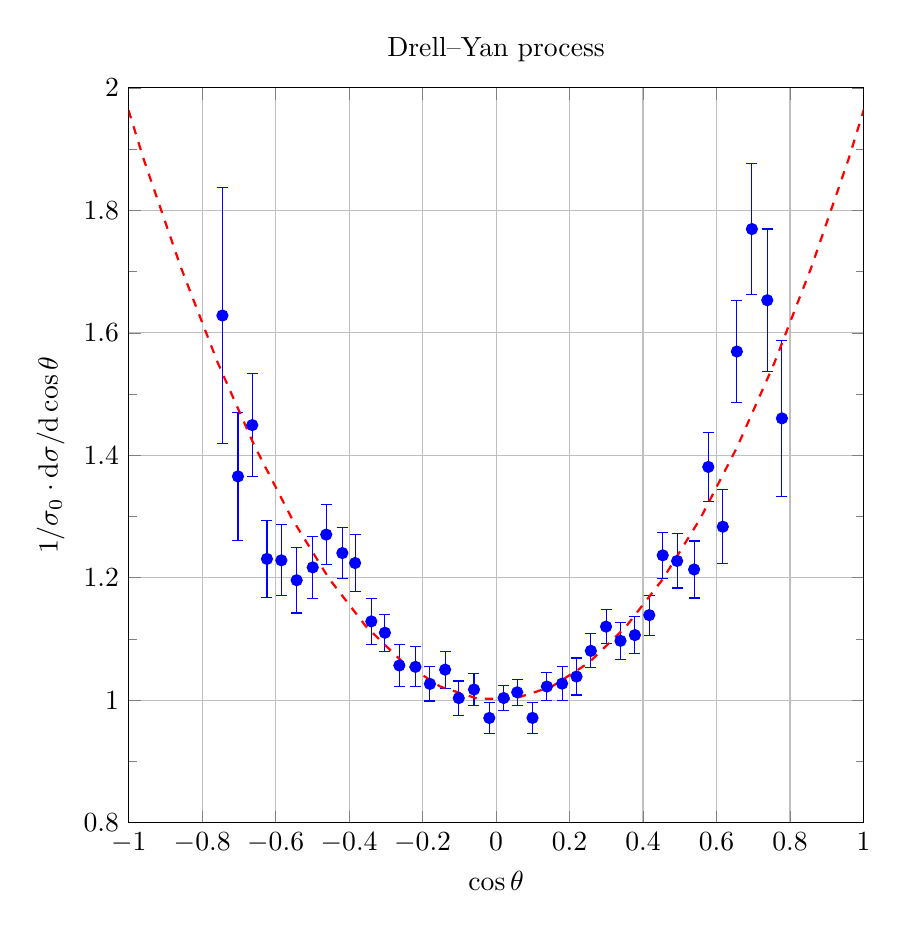
\begin{tikzpicture}[scale=1]
    \begin{axis}[
    width=0.9\textwidth,
    height=0.9\textwidth,
        title=Drell--Yan process,
        xlabel={$\cos\theta$},
        ylabel={$1/\sigma_0\cdot {\d\sigma}/{\d\cos\theta}$},
        xmin=-1, xmax=1,
        ymin = 0.8, ymax=2,
        minor y tick num=1,
        grid = major,
    ]
     \addplot[
    color=blue,
    only marks,mark=*,
    error bars/.cd,
    y dir=both, y explicit
    ]
    coordinates {
(-0.745026,1.628203)+-(0,0.209307)
(-0.702638,1.365462)+-(0,0.104651)
(-0.663698,1.449228)+-(0,0.083721)
(-0.623762,1.23067)+-(0,0.062793)
(-0.584539,1.22839)+-(0,0.058139)
(-0.542909,1.19588)+-(0,0.053489)
(-0.499149,1.216861)+-(0,0.05116)
(-0.462417,1.270393)+-(0,0.048837)
(-0.418488,1.240211)+-(0,0.041858)
(-0.383833,1.223972)+-(0,0.046514)
(-0.339689,1.128675)+-(0,0.037209)
(-0.302719,1.110113)+-(0,0.030233)
(-0.263327,1.056671)+-(0,0.034886)
(-0.219491,1.054396)+-(0,0.032555)
(-0.180183,1.026535)+-(0,0.027907)
(-0.138737,1.049839)+-(0,0.030229)
(-0.101675,1.00337)+-(0,0.027907)
(-0.060199,1.017372)+-(0,0.025581)
(-0.018523,0.970909)+-(0,0.025578)
(0.020585,1.003512)+-(0,0.020925)
(0.057463,1.012858)+-(0,0.02093)
(0.099123,0.971045)+-(0,0.025582)
(0.13817,1.022254)+-(0,0.023253)
(0.179677,1.026953)+-(0,0.027904)
(0.218854,1.038627)+-(0,0.030232)
(0.257932,1.080532)+-(0,0.027907)
(0.299324,1.120115)+-(0,0.027907)
(0.338616,1.096905)+-(0,0.030233)
(0.377801,1.106253)+-(0,0.030233)
(0.416909,1.138857)+-(0,0.032558)
(0.453496,1.236574)+-(0,0.037212)
(0.492742,1.227317)+-(0,0.044191)
(0.538924,1.213417)+-(0,0.046512)
(0.577588,1.380904)+-(0,0.055811)
(0.617125,1.283276)+-(0,0.060465)
(0.655398,1.569367)+-(0,0.083723)
(0.696262,1.769414)+-(0,0.106977)
(0.738167,1.653184)+-(0,0.116276)
(0.778019,1.460207)+-(0,0.127906)
};
        \addplot[thick,dashed,color=red,samples=100] { (1+0.96*x^2) };
  \end{axis}
\end{tikzpicture}%
\caption{Angular distribution of dilepton pairs in $p+Cu$ collisions at 800~GeV
measured by FNAL E772. The solid curve is a fit to $1+ \lambda \cos^2\theta$.
Data taken from
P.~McGaughey, ``{Recent measurements of quarkonia and Drell--Yan production in
  proton nucleus collisions},'' {\em Nucl. Phys. A}, vol.~610, pp.~394C--403C,
  1996.}
\end{figure}
%
%%%%%%%%%%%%%%%%   END FIGURE  %%%%%%%%%%%%%%%%%%%%%%%%%%%%%%
%
\end{document}
